\documentclass[10pt]{standalone}
\usepackage{pgf,tikz}
\usepackage{mathrsfs}
\usetikzlibrary{arrows}
\pagestyle{empty}
\begin{document}

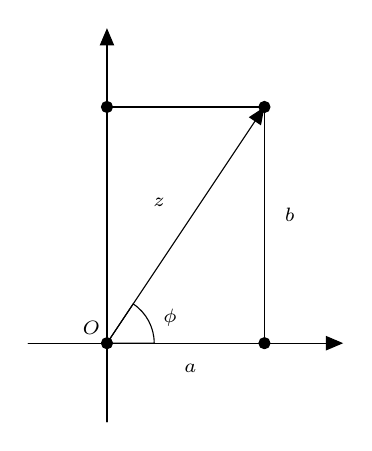
\begin{tikzpicture}[line cap=round,line join=round,>=triangle 45,x=1.0cm,y=1.0cm]
\draw[->] (-1.,0.) -- (3.,0.);

\draw[->] (0.,-1.) -- (0.,4.);

\clip(-1.,-1.) rectangle (3.,4.);
\draw [shift={(0.,0.)}] (0,0) -- (0.:0.6) arc (0.:56.309932474020215:0.6) -- cycle;
\draw [->] (0.,0.) -- (2.,3.);
\draw  (2.,3.)-- (2.,0.);
\draw  (2.,3.)-- (0.,3.);
\begin{scriptsize}
\draw [fill=black] (2.,3.) circle (2.0pt);

\draw [fill=black] (0.,0.) circle (2.0pt);
\draw (-0.2,0.2) node {$O$};
\draw (0.66,1.79) node {$z$};
\draw [fill=black] (2.,0.) circle (2.0pt);
\draw (2.32,1.63) node {$b$};
\draw [fill=black] (0.,3.) circle (2.0pt);
\draw (1.06,-.32) node {$a$};
\draw (.8,.32) node {$\phi$};
\end{scriptsize}
\end{tikzpicture}
\end{document}